\documentclass[14pt]{extbook}
\usepackage{multicol, enumerate, enumitem, hyperref, color, soul, setspace, parskip, fancyhdr} %General Packages
\usepackage{amssymb, amsthm, amsmath, latexsym, units, mathtools} %Math Packages
\everymath{\displaystyle} %All math in Display Style
% Packages with additional options
\usepackage[headsep=0.5cm,headheight=12pt, left=1 in,right= 1 in,top= 1 in,bottom= 1 in]{geometry}
\usepackage[usenames,dvipsnames]{xcolor}
\usepackage{dashrule}  % Package to use the command below to create lines between items
\newcommand{\litem}[1]{\item#1\hspace*{-1cm}\rule{\textwidth}{0.4pt}}
\pagestyle{fancy}
\lhead{Makeup Progress Quiz 3}
\chead{}
\rhead{Version ALL}
\lfoot{1648-1753}
\cfoot{}
\rfoot{Summer C 2021}
\begin{document}

\begin{enumerate}
\litem{
Determine the appropriate model for the graph of points below.
\begin{center}
    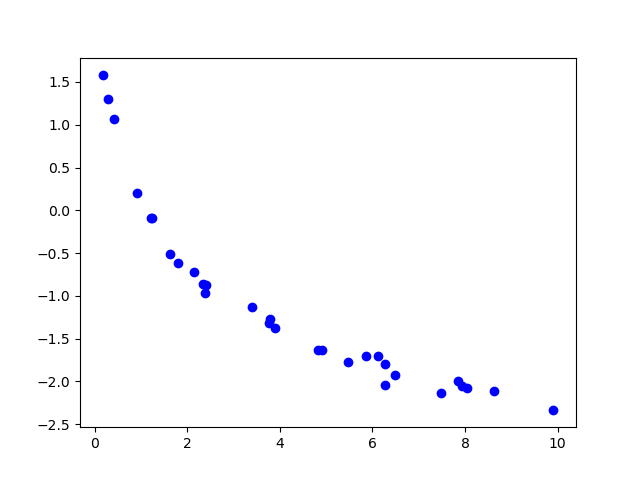
\includegraphics[width=0.5\textwidth]{../Figures/identifyModelGraph12A.png}
\end{center}
\begin{enumerate}[label=\Alph*.]
\item \( \text{Non-linear Power model} \)
\item \( \text{Exponential model} \)
\item \( \text{Linear model} \)
\item \( \text{Logarithmic model} \)
\item \( \text{None of the above} \)

\end{enumerate} }
\litem{
For the scenario below, use the model for the volume of a cylinder as $V = \pi r^2 h$.
\begin{center}
    \textit{ Pringles wants to add 38 \text{percent} more chips to their cylinder cans and minimize the design change of their cans. They've decided that the best way to minimize the design change is to increase the radius and height by the same percentage. What should this increase be? }
\end{center}
\begin{enumerate}[label=\Alph*.]
\item \( \text{About } 13 \text{ percent} \)
\item \( \text{About } 11 \text{ percent} \)
\item \( \text{About } 17 \text{ percent} \)
\item \( \text{About } 19 \text{ percent} \)
\item \( \text{None of the above} \)

\end{enumerate} }
\litem{
For the scenario below, use the model for the volume of a cylinder as $V = \pi r^2 h$.
\begin{center}
    \textit{ Pringles wants to add 43 \text{percent} more chips to their cylinder cans and minimize the design change of their cans. They've decided that the best way to minimize the design change is to increase the radius and height by the same percentage. What should this increase be? }
\end{center}
\begin{enumerate}[label=\Alph*.]
\item \( \text{About } 13 \text{ percent} \)
\item \( \text{About } 22 \text{ percent} \)
\item \( \text{About } 20 \text{ percent} \)
\item \( \text{About } 4 \text{ percent} \)
\item \( \text{None of the above} \)

\end{enumerate} }
\litem{
Determine the appropriate model for the graph of points below.
\begin{center}
    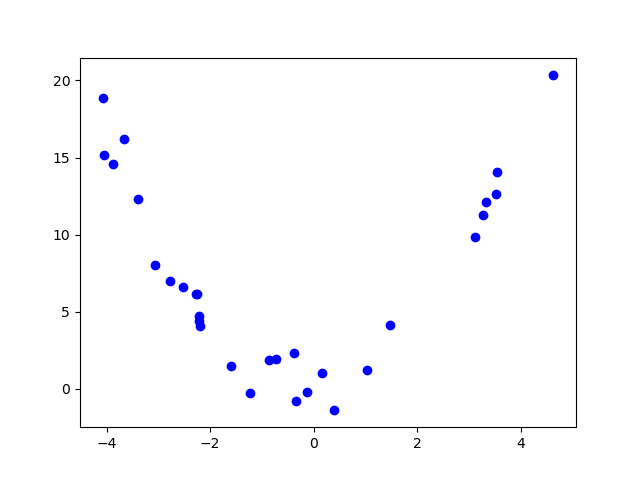
\includegraphics[width=0.5\textwidth]{../Figures/identifyModelGraph12CopyA.png}
\end{center}
\begin{enumerate}[label=\Alph*.]
\item \( \text{Linear model} \)
\item \( \text{Exponential model} \)
\item \( \text{Non-linear Power model} \)
\item \( \text{Logarithmic model} \)
\item \( \text{None of the above} \)

\end{enumerate} }
\litem{
Solve the modeling problem below, if possible.
\begin{center}
    \textit{ A new virus is spreading throughout the world. There were initially 4 many cases reported, but the number of confirmed cases has doubled every 1 days. How long will it be until there are at least 100000 confirmed cases? }
\end{center}
\begin{enumerate}[label=\Alph*.]
\item \( \text{About } 6 \text{ days} \)
\item \( \text{About } 5 \text{ days} \)
\item \( \text{About } 15 \text{ days} \)
\item \( \text{About } 11 \text{ days} \)
\item \( \text{There is not enough information to solve the problem.} \)

\end{enumerate} }
\litem{
Solve the modeling problem below, if possible.
\begin{center}
    \textit{ In CHM2045L, Brittany created a 25 liter 23 percent solution of chemical $\chi$ using two different solution percentages of chemical $\chi$. When she went to write her lab report, she realized she forgot to write the amount of each solution she used! If she remembers she used 17 percent and 32 percent solutions, what was the amount she used of the 17 percent solution? }
\end{center}
\begin{enumerate}[label=\Alph*.]
\item \( 12.50 liters \)
\item \( 12.79 liters \)
\item \( 15.00 liters \)
\item \( 10.00 liters \)
\item \( \text{There is not enough information to solve the problem.} \)

\end{enumerate} }
\litem{
Solve the modeling problem below, if possible.
\begin{center}
    \textit{ In CHM2045L, Brittany created a 16 liter 34 percent solution of chemical $\chi$ using two different solution percentages of chemical $\chi$. When she went to write her lab report, she realized she forgot to write the amount of each solution she used! If she remembers she used 13 percent and 39 percent solutions, what was the amount she used of the 39 percent solution? }
\end{center}
\begin{enumerate}[label=\Alph*.]
\item \( 12.92 liters \)
\item \( 3.08 liters \)
\item \( 7.91 liters \)
\item \( 8.00 liters \)
\item \( \text{There is not enough information to solve the problem.} \)

\end{enumerate} }
\litem{
For the information below, construct a linear model that describes the total time $T$ spent on the path in terms of the distance of a particular part of the path \textit{if we know that the time spent on each path was equal}.
\begin{center}
    \textit{ A bicyclist is training for a race on a hilly path. Their bike keeps track of their speed at any time, but not the distance traveled. Their speed traveling up a hill is 6 mph, 12 mph when traveling down a hill, and 8 mph when traveling along a flat portion. }
\end{center}
\begin{enumerate}[label=\Alph*.]
\item \( 576.000 D \)
\item \( 0.375 D \)
\item \( 26.000 D \)
\item \( \text{The model can be found with the information provided, but isn't options 1-3.} \)
\item \( \text{The model cannot be found with the information provided.} \)

\end{enumerate} }
\litem{
The temperature of an object, $T$, in a different surrounding temperature $T_s$ will behave according to the formula $T(t) = Ae^{kt} + T_s$, where $t$ is minutes, $A$ is a constant, and k is a constant. Use this formula and the situation below to construct a model that describes the uranium's temperature, $T$, based on the amount of time t (in minutes) that have passed. Choose the correct constant $k$ from the options below.
\begin{center}
    \textit{ Uranium is taken out of the reactor with a temperature of $130^{\circ}$ C and is placed into a $20^{\circ}$ C bath to cool. After 19 minutes, the uranium has cooled to $85^{\circ}$ C. }
\end{center}
\begin{enumerate}[label=\Alph*.]
\item \( k = -0.03648 \)
\item \( k = -0.03854 \)
\item \( k = -0.03744 \)
\item \( k = -0.02769 \)
\item \( \text{None of the above} \)

\end{enumerate} }
\litem{
Solve the modeling problem below, if possible.
\begin{center}
    \textit{ A new virus is spreading throughout the world. There were initially 6 many cases reported, but the number of confirmed cases has doubled every 4 days. How long will it be until there are at least 1000000 confirmed cases? }
\end{center}
\begin{enumerate}[label=\Alph*.]
\item \( \text{About } 20 \text{ days} \)
\item \( \text{About } 70 \text{ days} \)
\item \( \text{About } 49 \text{ days} \)
\item \( \text{About } 23 \text{ days} \)
\item \( \text{There is not enough information to solve the problem.} \)

\end{enumerate} }
\litem{
Determine the appropriate model for the graph of points below.
\begin{center}
    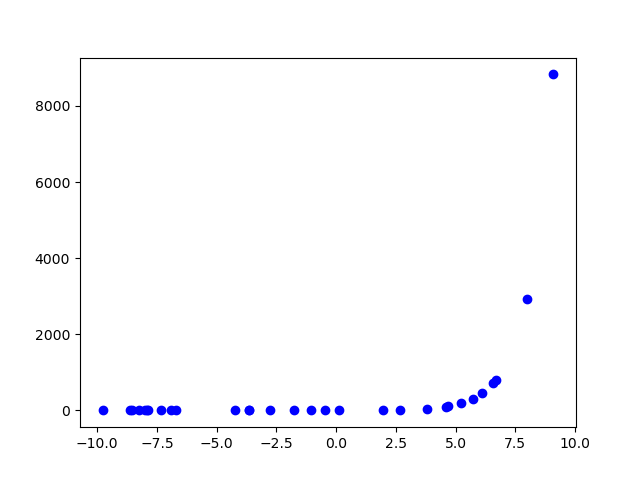
\includegraphics[width=0.5\textwidth]{../Figures/identifyModelGraph12B.png}
\end{center}
\begin{enumerate}[label=\Alph*.]
\item \( \text{Exponential model} \)
\item \( \text{Logarithmic model} \)
\item \( \text{Linear model} \)
\item \( \text{Non-linear Power model} \)
\item \( \text{None of the above} \)

\end{enumerate} }
\litem{
For the scenario below, use the model for the volume of a cylinder as $V = \pi r^2 h$.
\begin{center}
    \textit{ Pringles wants to add 27 \text{percent} more chips to their cylinder cans and minimize the design change of their cans. They've decided that the best way to minimize the design change is to increase the radius and height by the same percentage. What should this increase be? }
\end{center}
\begin{enumerate}[label=\Alph*.]
\item \( \text{About } 3 \text{ percent} \)
\item \( \text{About } 14 \text{ percent} \)
\item \( \text{About } 13 \text{ percent} \)
\item \( \text{About } 8 \text{ percent} \)
\item \( \text{None of the above} \)

\end{enumerate} }
\litem{
For the scenario below, use the model for the volume of a cylinder as $V = \pi r^2 h$.
\begin{center}
    \textit{ Pringles wants to add 27 \text{percent} more chips to their cylinder cans and minimize the design change of their cans. They've decided that the best way to minimize the design change is to increase the radius and height by the same percentage. What should this increase be? }
\end{center}
\begin{enumerate}[label=\Alph*.]
\item \( \text{About } 8 \text{ percent} \)
\item \( \text{About } 13 \text{ percent} \)
\item \( \text{About } 3 \text{ percent} \)
\item \( \text{About } 14 \text{ percent} \)
\item \( \text{None of the above} \)

\end{enumerate} }
\litem{
Determine the appropriate model for the graph of points below.
\begin{center}
    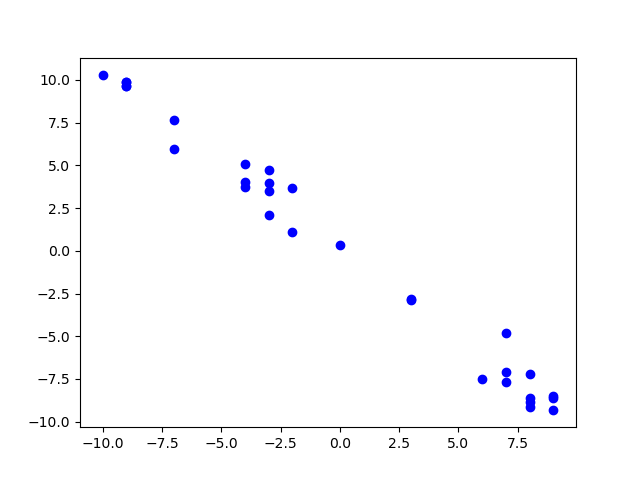
\includegraphics[width=0.5\textwidth]{../Figures/identifyModelGraph12CopyB.png}
\end{center}
\begin{enumerate}[label=\Alph*.]
\item \( \text{Non-linear Power model} \)
\item \( \text{Linear model} \)
\item \( \text{Exponential model} \)
\item \( \text{Logarithmic model} \)
\item \( \text{None of the above} \)

\end{enumerate} }
\litem{
Solve the modeling problem below, if possible.
\begin{center}
    \textit{ A new virus is spreading throughout the world. There were initially 3 many cases reported, but the number of confirmed cases has quadrupled every 1 days. How long will it be until there are at least 100000 confirmed cases? }
\end{center}
\begin{enumerate}[label=\Alph*.]
\item \( \text{About } 5 \text{ days} \)
\item \( \text{About } 8 \text{ days} \)
\item \( \text{About } 11 \text{ days} \)
\item \( \text{About } 6 \text{ days} \)
\item \( \text{There is not enough information to solve the problem.} \)

\end{enumerate} }
\litem{
Solve the modeling problem below, if possible.
\begin{center}
    \textit{ In CHM2045L, Brittany created a 24 liter 14 percent solution of chemical $\chi$ using two different solution percentages of chemical $\chi$. When she went to write her lab report, she realized she forgot to write the amount of each solution she used! If she remembers she used 8 percent and 19 percent solutions, what was the amount she used of the 8 percent solution? }
\end{center}
\begin{enumerate}[label=\Alph*.]
\item \( 11.65 liters \)
\item \( 12.00 liters \)
\item \( 13.09 liters \)
\item \( 10.91 liters \)
\item \( \text{There is not enough information to solve the problem.} \)

\end{enumerate} }
\litem{
Solve the modeling problem below, if possible.
\begin{center}
    \textit{ In CHM2045L, Brittany created a 27 liter 27 percent solution of chemical $\chi$ using two different solution percentages of chemical $\chi$. When she went to write her lab report, she realized she forgot to write the amount of each solution she used! If she remembers she used 10 percent and 36 percent solutions, what was the amount she used of the 36 percent solution? }
\end{center}
\begin{enumerate}[label=\Alph*.]
\item \( 12.68 liters \)
\item \( 9.35 liters \)
\item \( 13.50 liters \)
\item \( 17.65 liters \)
\item \( \text{There is not enough information to solve the problem.} \)

\end{enumerate} }
\litem{
For the scenario below, find the variation constant $k$ of the model (if possible).
\begin{center}
    \textit{ In an alternative galaxy, the square of the time, $T$ (Earth years), required for a planet to orbit Sun $\chi$ increases as the square of the distance, $d$ (AUs), that the planet is from Sun $\chi$ increases. For example, when Ea's average distance from Sun $\chi$ is 7, it takes 100 Earth days to complete an orbit. }
\end{center}
\begin{enumerate}[label=\Alph*.]
\item \( k = 490000.000 \)
\item \( k = 4.028 \)
\item \( k = 204.082 \)
\item \( k = 3.780 \)
\item \( \text{Unable to compute the constant based on the information given.} \)

\end{enumerate} }
\litem{
For the information provided below, construct a linear model that describes her total costs, $C$, as a function of the number of months, $x$ she is at UF. 
\begin{center}
    \textit{ Aubrey is a college student going into her first year at UF. She will receive Bright Futures, which covers her tuition plus a \$600 educational expense each year. Before college, Aubrey saved up \$10000. She knows she will need to pay \$1200 in rent a month, \$80 for food a week, and \$40 in other weekly expenses. }
\end{center}
\begin{enumerate}[label=\Alph*.]
\item \( C(x) = 1320 x \)
\item \( C(x) = 10600 \)
\item \( C(x) = 1320 \)
\item \( C(x) = 10600 x \)
\item \( \text{None of the above.} \)

\end{enumerate} }
\litem{
Solve the modeling problem below, if possible.
\begin{center}
    \textit{ A new virus is spreading throughout the world. There were initially 4 many cases reported, but the number of confirmed cases has tripled every 5 days. How long will it be until there are at least 10000 confirmed cases? }
\end{center}
\begin{enumerate}[label=\Alph*.]
\item \( \text{About } 19 \text{ days} \)
\item \( \text{About } 36 \text{ days} \)
\item \( \text{About } 40 \text{ days} \)
\item \( \text{About } 20 \text{ days} \)
\item \( \text{There is not enough information to solve the problem.} \)

\end{enumerate} }
\litem{
Determine the appropriate model for the graph of points below.
\begin{center}
    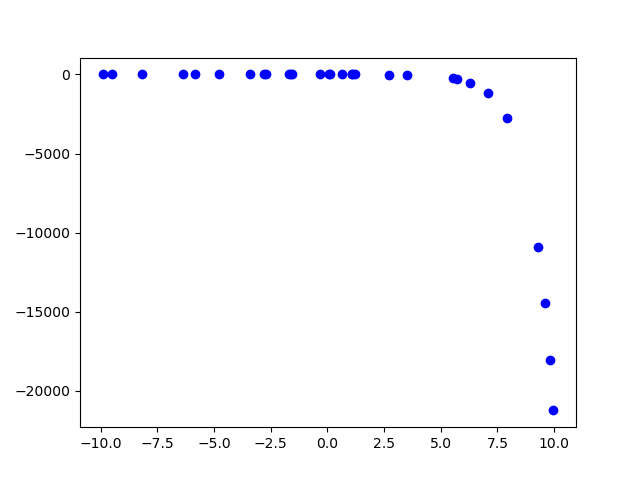
\includegraphics[width=0.5\textwidth]{../Figures/identifyModelGraph12C.png}
\end{center}
\begin{enumerate}[label=\Alph*.]
\item \( \text{Non-linear Power model} \)
\item \( \text{Logarithmic model} \)
\item \( \text{Linear model} \)
\item \( \text{Exponential model} \)
\item \( \text{None of the above} \)

\end{enumerate} }
\litem{
For the scenario below, use the model for the volume of a cylinder as $V = \pi r^2 h$.
\begin{center}
    \textit{ Pringles wants to add 28 \text{percent} more chips to their cylinder cans and minimize the design change of their cans. They've decided that the best way to minimize the design change is to increase the radius and height by the same percentage. What should this increase be? }
\end{center}
\begin{enumerate}[label=\Alph*.]
\item \( \text{About } 3 \text{ percent} \)
\item \( \text{About } 13 \text{ percent} \)
\item \( \text{About } 9 \text{ percent} \)
\item \( \text{About } 14 \text{ percent} \)
\item \( \text{None of the above} \)

\end{enumerate} }
\litem{
For the scenario below, use the model for the volume of a cylinder as $V = \pi r^2 h$.
\begin{center}
    \textit{ Pringles wants to add 34 \text{percent} more chips to their cylinder cans and minimize the design change of their cans. They've decided that the best way to minimize the design change is to increase the radius and height by the same percentage. What should this increase be? }
\end{center}
\begin{enumerate}[label=\Alph*.]
\item \( \text{About } 11 \text{ percent} \)
\item \( \text{About } 16 \text{ percent} \)
\item \( \text{About } 17 \text{ percent} \)
\item \( \text{About } 10 \text{ percent} \)
\item \( \text{None of the above} \)

\end{enumerate} }
\litem{
Determine the appropriate model for the graph of points below.
\begin{center}
    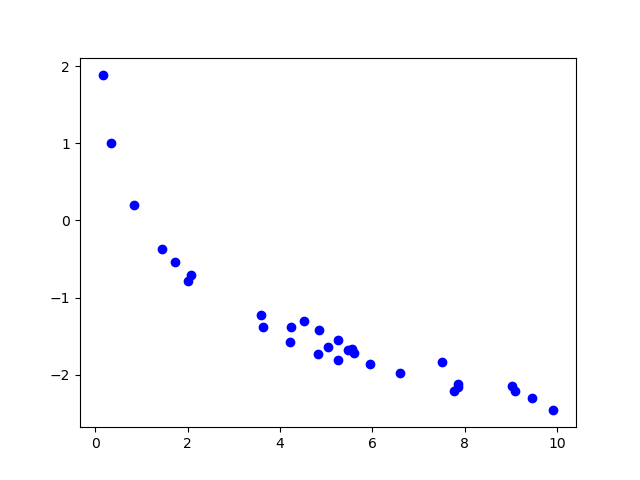
\includegraphics[width=0.5\textwidth]{../Figures/identifyModelGraph12CopyC.png}
\end{center}
\begin{enumerate}[label=\Alph*.]
\item \( \text{Non-linear Power model} \)
\item \( \text{Exponential model} \)
\item \( \text{Linear model} \)
\item \( \text{Logarithmic model} \)
\item \( \text{None of the above} \)

\end{enumerate} }
\litem{
Solve the modeling problem below, if possible.
\begin{center}
    \textit{ A new virus is spreading throughout the world. There were initially 3 many cases reported, but the number of confirmed cases has doubled every 5 days. How long will it be until there are at least 10000 confirmed cases? }
\end{center}
\begin{enumerate}[label=\Alph*.]
\item \( \text{About } 26 \text{ days} \)
\item \( \text{About } 41 \text{ days} \)
\item \( \text{About } 59 \text{ days} \)
\item \( \text{About } 22 \text{ days} \)
\item \( \text{There is not enough information to solve the problem.} \)

\end{enumerate} }
\litem{
Solve the modeling problem below, if possible.
\begin{center}
    \textit{ In CHM2045L, Brittany created a 17 liter 33 percent solution of chemical $\chi$ using two different solution percentages of chemical $\chi$. When she went to write her lab report, she realized she forgot to write the amount of each solution she used! If she remembers she used 19 percent and 45 percent solutions, what was the amount she used of the 19 percent solution? }
\end{center}
\begin{enumerate}[label=\Alph*.]
\item \( 7.85 liters \)
\item \( 9.15 liters \)
\item \( 8.50 liters \)
\item \( 8.43 liters \)
\item \( \text{There is not enough information to solve the problem.} \)

\end{enumerate} }
\litem{
Solve the modeling problem below, if possible.
\begin{center}
    \textit{ In CHM2045L, Brittany created a 22 liter 19 percent solution of chemical $\chi$ using two different solution percentages of chemical $\chi$. When she went to write her lab report, she realized she forgot to write the amount of each solution she used! If she remembers she used 17 percent and 40 percent solutions, what was the amount she used of the 17 percent solution? }
\end{center}
\begin{enumerate}[label=\Alph*.]
\item \( 1.91 liters \)
\item \( 11.00 liters \)
\item \( 16.54 liters \)
\item \( 20.09 liters \)
\item \( \text{There is not enough information to solve the problem.} \)

\end{enumerate} }
\litem{
Using the scenario below, model the population of bacteria $\alpha$ in terms of the number of minutes, $t$ that pass. Then, choose the correct approximate \textit{(rounded to the nearest minute)} replication rate of bacteria-$\alpha$.
\begin{center}
    \textit{ A newly discovered bacteria, $\alpha$, is being examined in a lab. The lab started with a petri dish of 2 bacteria-$\alpha$. After 3 hours, the petri dish has 855 bacteria-$\alpha$. Based on similar bacteria, the lab believes bacteria-$\alpha$ doubles after some undetermined number of minutes. }
\end{center}
\begin{enumerate}[label=\Alph*.]
\item \( \text{About } 20 \text{ minutes} \)
\item \( \text{About } 221 \text{ minutes} \)
\item \( \text{About } 36 \text{ minutes} \)
\item \( \text{About } 123 \text{ minutes} \)
\item \( \text{None of the above} \)

\end{enumerate} }
\litem{
For the scenario below, model the rate of vibration (cm/s) of the string in terms of the length of the string. Then determine the variation constant $k$ of the model (if possible). The constant should be in terms of cm and s.
\begin{center}
    \textit{ The rate of vibration of a string under constant tension varies based on the type of string and the length of the string. The rate of vibration of string $\omega$ decreases as the cube length of the string increases. For example, when string $\omega$ is 2 mm long, the rate of vibration is 21 cm/s. }
\end{center}
\begin{enumerate}[label=\Alph*.]
\item \( k = 2625.00 \)
\item \( k = 0.17 \)
\item \( k = 168.00 \)
\item \( k = 2.62 \)
\item \( \text{None of the above.} \)

\end{enumerate} }
\litem{
Solve the modeling problem below, if possible.
\begin{center}
    \textit{ A new virus is spreading throughout the world. There were initially 8 many cases reported, but the number of confirmed cases has quadrupled every 1 days. How long will it be until there are at least 1000000 confirmed cases? }
\end{center}
\begin{enumerate}[label=\Alph*.]
\item \( \text{About } 9 \text{ days} \)
\item \( \text{About } 12 \text{ days} \)
\item \( \text{About } 5 \text{ days} \)
\item \( \text{About } 4 \text{ days} \)
\item \( \text{There is not enough information to solve the problem.} \)

\end{enumerate} }
\end{enumerate}

\end{document}